\chapter{Tools and Interoperability} % Main chapter title

\label{Chapter7} % Change X to a consecutive number; for referencing this chapter elsewhere, use \ref{ChapterX}

\lhead{Chapter 7. \emph{Tools and Interoperability}} % Change X to a consecutive number; this is for the header on each page - perhaps a shortened title

%----------------------------------------------------------------------------------------
%	SECTION 1
%----------------------------------------------------------------------------------------

% Solibri…
% Include other ``tools/ technologies" as they are called by Fred, e.g. IFC, COBie (?)?
% Revit.
% Bluebeam Revu.

\section{BIM Software Providers}

The market-leading BIM software providers are Autodesk, Bentley, Nemetschek, and Trimble \citep{Bosche, BusinessWire}.
The most commonly used software programme for building services engineers in the UK is Autodesk Revit MEP.

%----------------------------------------------------------------------------------------
%	SECTION 2
%----------------------------------------------------------------------------------------


\section{Problems of Interoperability}
% Part of the root of these problems is the lack of interoperability due to weakly coordinated market demand for standards e.g. IFC.
Interoperability is the ability of different software applications to exchange and make use of data \citep{Gallaher2004}.
The benefit of interoperability is illustrated in Figure \ref{io}. If no common open standard exists, each individual software application must develop and implement direct translators back and forth for all other pieces of software which it seeks to communicate with. If an open standard can be used instead, the mappings only need to be translated back and forth from that single format in order to be compatible with all other applications supporting the same standard \citep{Laakso2012}.
\cite{Laakso2012} explain that it might seem natural for a user to adopt an open format, considering its theoretical benefits.
But, as an anecdotal example shows, this is not always the case.
Free and open word processing software applications have been available for several years, and yet the Microsoft Word file format (a vendor-specific proprietary format) continues to be perceived as the de-facto standard format.

\begin{figure}[htbp]
	\centering
	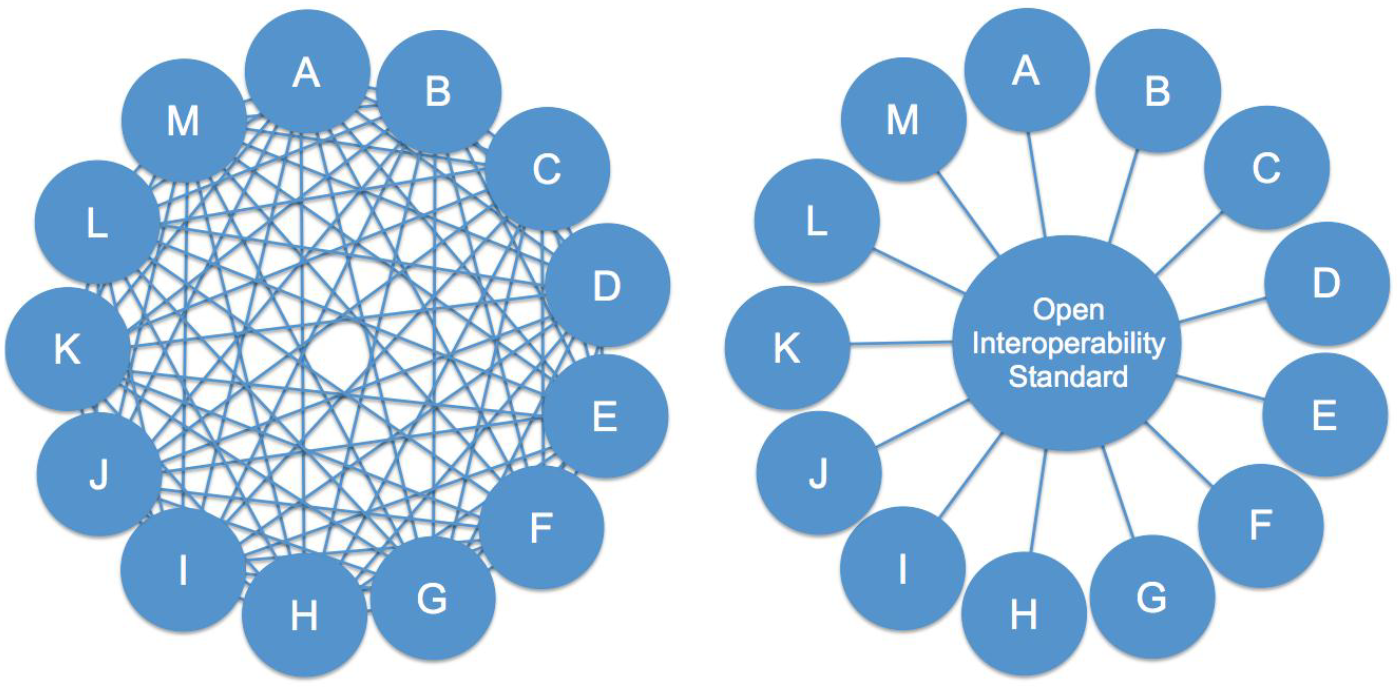
\includegraphics[width=\textwidth]{figures/Interoperability.png}
	\rule{\textwidth}{0.5pt} % use line???
	\caption[Direct translators between software applications vs. an open interoperability standard]{Direct translators between software applications vs. an open interoperability standard \citep{Laakso2012}.}
	\label{io}
\end{figure}

The Industry Foundation Classes (IFC) are an open, internationally recognised and standardised data model that is intended to enable interoperability between BIM software applications \citep{Laakso2012}.
The origins of IFC date back to the early 1990s \citep{Laakso2012}.
Considering that the first BIM software to be made available on a personal computer was released in 1984 \citep{Quirk2012}, IFC developed relatively early.
According to \cite{Laakso2012}, buildingSMART (the developer of IFC) wished to standardise IFC during the early stages of BIM so that IFC could be implemented into the new BIM software applications entering the marketplace, thus preventing proprietary solutions from gaining dominance.
This plan unfortunately did not work specifically due to the low market demand for BIM technologies in the early stages, thus making it challenging to get sufficient resources to manage the development of the IFC standard.
As a result, the exchange of BIM data has been dominated by proprietary solutions.
Moreover, although IFC has been around for a relatively long time and even been implemented into leading BIM software, actual use of IFC as an enabler of interoperability has been slow but steadily increasing \citep{Laakso2012}.
